\documentclass[10.5pt]{article}

% ACL style package
\usepackage{acl}

% Standard packages
\usepackage{times}
\usepackage{latexsym}
\usepackage[T1]{fontenc}
\usepackage[utf8]{inputenc}
\usepackage{graphicx}
\usepackage{amsmath}
\usepackage{booktabs}
\usepackage{siunitx}
\usepackage{tabularx}
\usepackage{multirow}
\usepackage{ragged2e}

\title{The Role of Data Variety: Observing Cross-Skill Impacts Through Targeted LLM Unlearning}
\author{William Chastek \\ Joseph V. \\ John Phan \\
Team Name: NoobLP}

\begin{document}
\maketitle

\begin{abstract}
Large Language Models (LLMs) excel in multi-task reasoning, but their ability to selectively "unlearn" specific skills without degrading unrelated capabilities remains poorly understood. This study investigates the cross-domain impacts of unlearning mathematical reasoning in the DeepSeek-R1-Distill-Queen-1.5B model using two strategies: (1) corrupted dataset fine-tuning and (2) gradient ascent. Results show a 12.7\% average accuracy drop in math tasks, with collateral degradation in reasoning (9.2\%) and data analysis (6.8\%). Gradient ascent caused the steepest math accuracy decline (18.65\%) but minimized impacts on coding (-3.1\%) and language comprehension (-2.4\%). Our findings highlight the interconnectedness of LLM skills and advocate for domain-specific unlearning protocols.
\end{abstract}

\section{Introduction}
LLM unlearning has been a topic of interest since the development of very large LLM platforms such as ChatGPT, as a way to remove unwanted behaviors. In this context, “unlearning” pertains to modifying the model weights to forget a concept or skill. Currently, researchers used a combination of reinforcement learning\cite{mu2024rule}, as well as gradient ascent\cite{neel2020descenttodeletegradientbasedmethodsmachine} to unlearn unwanted behaviors or knowledge. Many reinforcement learning techniques require human input, which makes it hard to scale and gradient ascent approaches have shown to cause degradation in LLM performance outside of the unwanted behavior or knowledge. 

\section{Motivation}
Unlearning techniques are critical for adapting LLMs to evolving ethical and practical standards. However, unintended skill degradation poses risks—for instance, unlearning math might impair logical reasoning or data analysis. This work addresses two questions:
\begin{enumerate}
    \item How does unlearning a specific skill affect performance in related domains?
    \item Can unlearning methods be refined to minimize collateral damage?
\end{enumerate}

\section{Datasets and Models}
\subsection{Models}
The model used for experimentation was DeepSeek-R1-Distill-Qwen-1.5B from HuggingFace.
\subsection{Datasets}
\begin{itemize}
  \item \textbf{Training:} MATH\_algebra\_crowdsourced (AllenAI/LILA) \cite{mishra2022lila}.
  \item \textbf{Evaluation:} Math500 subset of PRM \cite{lightman2023lets}; LiveBench benchmark with six skill categories.
\end{itemize}
The MATH\_algebra\_crowdsourced dataset consists of 263 algebra problems, along with reasoning and the correct answer for each question. The Math500 dataset much like the 
\\MATH\_algebra\_crowdsourced dataset, consists of 500 math questions along with reasoning and the correct answer for each question, with the addition of a subject field for each question.
\\
The MATH\_algebra\_crowdsourced dataset was chosen for fine-tuning because it consists of only algebra questions, as we are interesting focused unlearning on number heavy math. While the Math500 dataset was chosen to showcase the accuracy the models get on different fields of math.

\section{Approach}
There are two phases to the project:

\subsection{Training}
The unlearning process was conducted in two different ways:
\begin{enumerate}
    \item \textbf{Corrupted Dataset:} Fine-tune the model on a corrupted or scrambled dataset.
    \item \textbf{Gradient Ascent:} Fine-tune the model on the original math dataset using gradient ascent to push the model away from correct math answers.
\end{enumerate}
\\
The corrupted dataset has three variants:
\begin{enumerate}
    \item \textbf{scrambled:} Answers are swapped across items so none remain correct.
    \item \textbf{val-modified:} Non-question numbers are modified but retain original digit lengths.
    \item \textbf{length-val-modified:} Non-question numbers are modified and digit lengths may change.
\end{enumerate}
The base DeepSeek-R1-Distill-Queen-1.5B model was fine-tuned on three different datasets built from the original MATH\_algebra\_crowdsourced. For each item in the dataset, the ''output\_answer'' section was corrupted.
\\
Gradient ascent has two variants:
\begin{enumerate}
    \item \textbf{gradient-ascent:} Use the negative loss for ascent.
    \item \textbf{reduced-eos-gradient-ascent:} Same as gradient-ascent but reduce EOS token priority to discourage early stopping.
\end{enumerate}
\subsubsection{Hyperparameters}
The hyperparameters for the training loop were:
\begin{enumerate}
    \item Number of Epochs: 1
    \item Learning Rate: $2e^{-5}$
    \item Batch Size: 1
    \item Weight Decay: 0.01
    \item Precision: float16
\end{enumerate}
Each model, was finetuned using this prompt template\begin{verbatim}
    ‘Please reason step by step, and 
    put your final answer within 
    \boxed{}.\n{problem_text}’
\end{verbatim} 
and trained to minimize the loss, with the excpetion of the gradient ascent models which were trained to maximize the loss.
\subsection{Testing}
We used the LiveBench LLM benchmark~\cite{livebench}, which covers six categories, and the Math500 dataset~\cite{lightman2023lets} to evaluate cross-domain effects. Two prompt templates were used for evaluation on the Math500 and MATH\_algebra\_crowdsourced dataset:
\begin{enumerate}
    \item \textbf{Chain-of-Thought Prompting:}
    \begin{verbatim}
Please reason step by step, 
and put your final answer 
within \boxed{}. {problem_text}
    \end{verbatim}
    \item \textbf{Direct Prompting:}
    \begin{verbatim}
{problem_text}. Place your 
final answer in a box 
with \boxed{}
    \end{verbatim}
\end{enumerate}
Additionally for the Math500 dataset, a temperature of 0.6 was used, and the models had a maximum of 8192 token sequence length. In total seven models were tested. Five of which were created using the methods described above. The other two were the base model from HuggingFace, as well as a model fine-tuned on the original MATH\_algebra\_crowdsourced dataset. These seven models were then benchmarked to see the performance between them.


\section{Experiments and Results}
To see if the unlearning was successful, the original non-corrupted dataset was used for evaluation. Using the two prompt templates, Chain-of-Though(CoT) and direct prompting, for evaluation, the accuracy for each model was recorded in Figure 1 and Figure 2. 
\\
\begin{figure}[h]
    \centering
    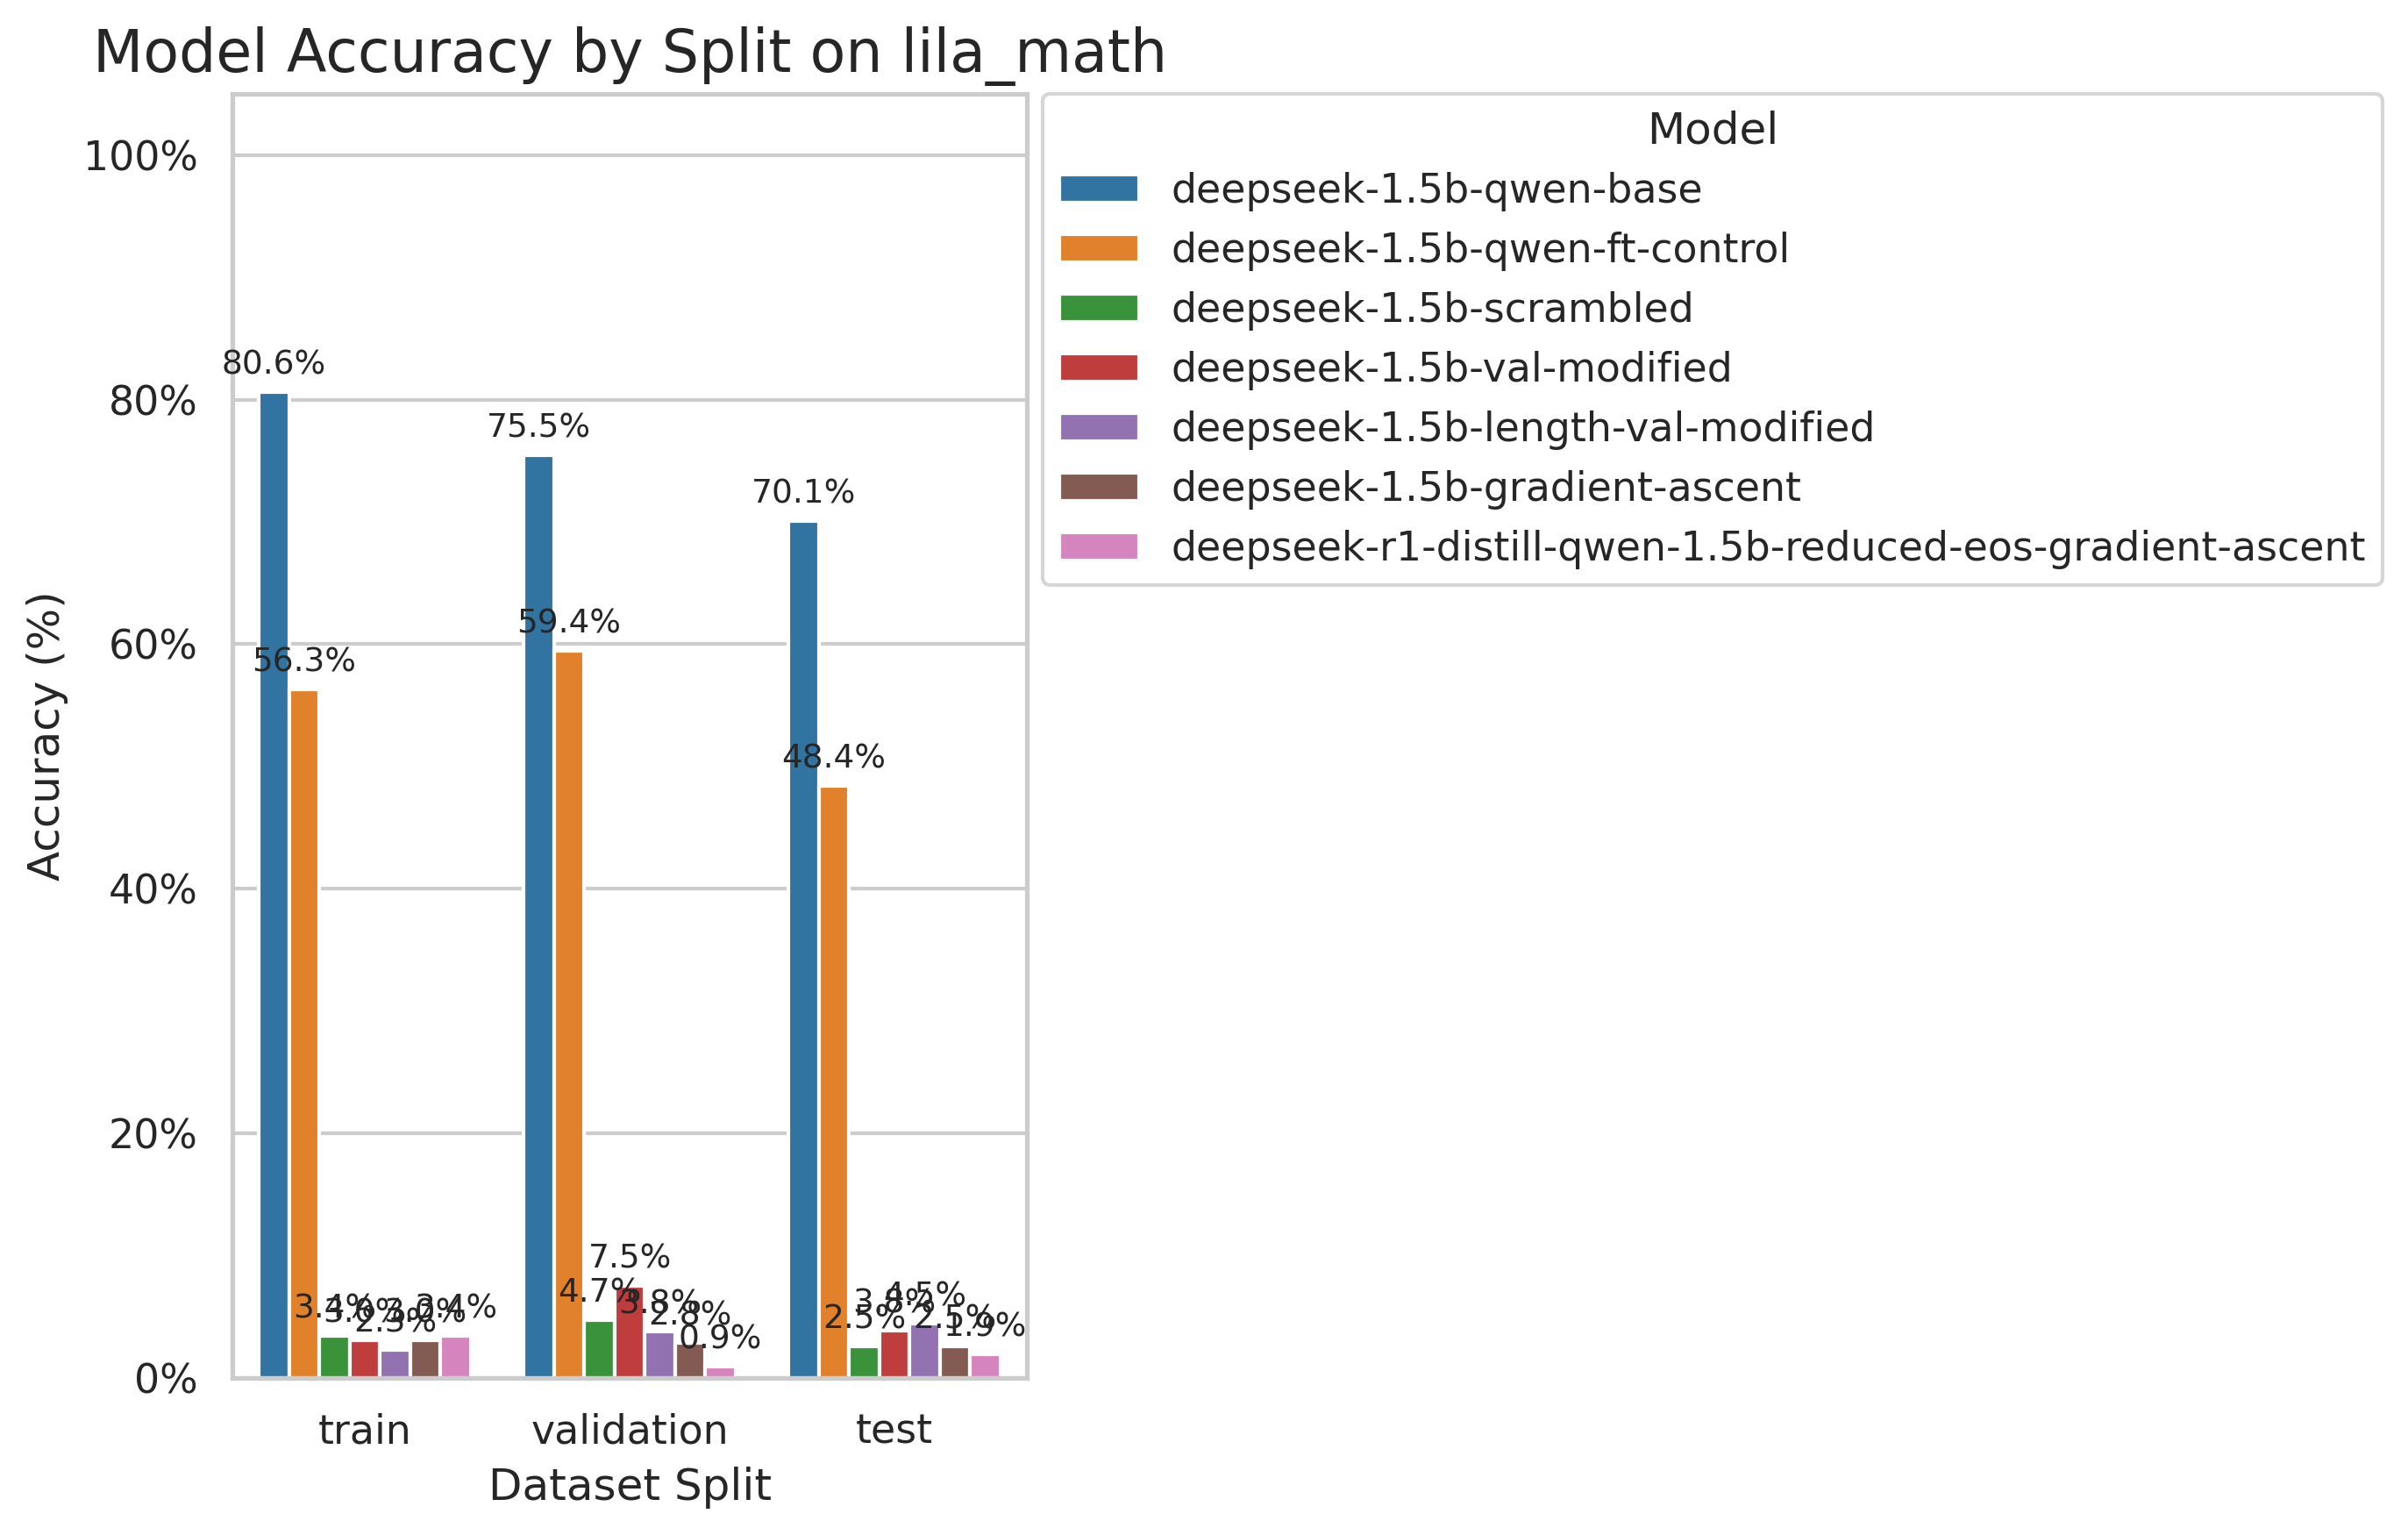
\includegraphics[width=1\linewidth]{main_prompt_lila_math_accuracy_by_split_20250504_230401.png}
    \caption{Model accuracy on original non-corrupted dataset used for finetuning using CoT prompting}
    \label{fig:enter-label}
\end{figure}
\begin{figure}[h]
    \centering
    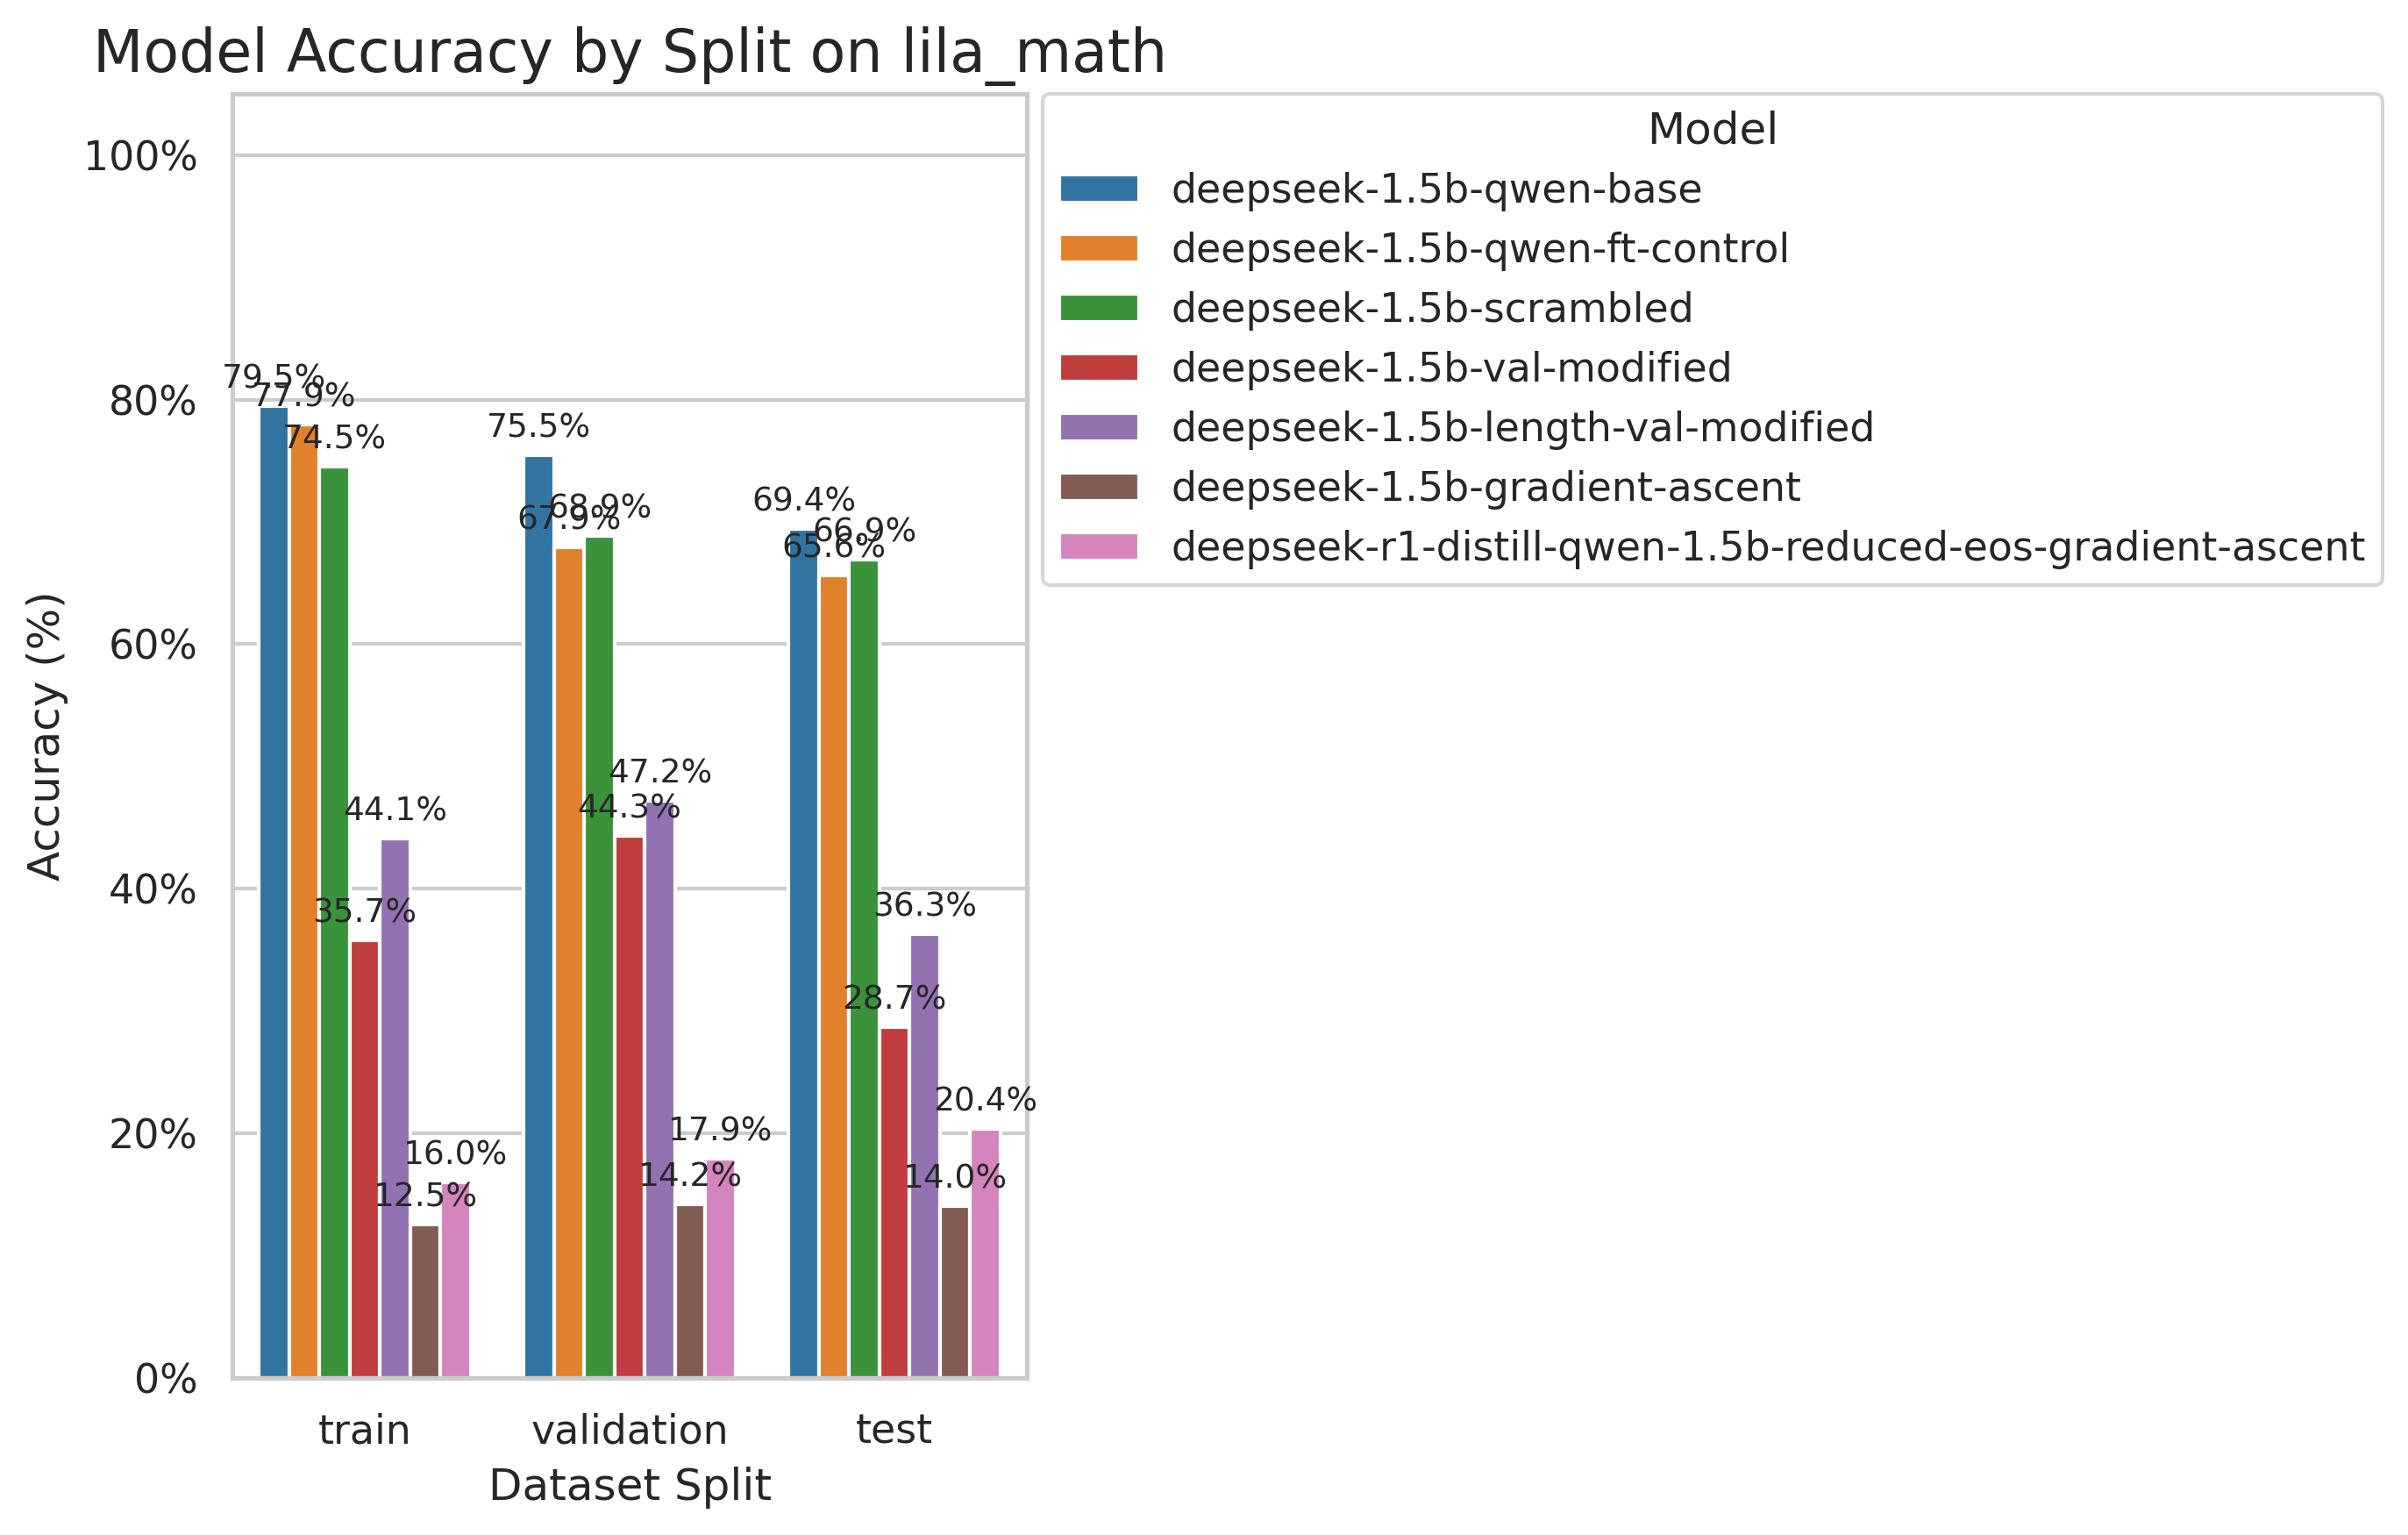
\includegraphics[width=1\linewidth]{new_prompt_lila_math_accuracy_by_split_20250505_192457.png}
    \caption{Model accuracy on original non-corrupted dataset used for finetuning using no CoT prompting}
    \label{fig:enter-label}
\end{figure}
As depicted in Figure 1 and 2, there is a large difference between CoT prompting and direct prompting. Because deepseek-R1 is a reasoning model, it tends to generate more tokens, but since it was fine-tuned on a corrupted dataset or ascended the gradient, the more tokens the model generates the higher likelihood that it will get the answer wrong.
\\
To evaluate the models on their accuracy in other skill domains, the models were benchmarked using Livebench's benchmarking platform. This benchmark tests the models capabilities in six different fields: coding, data analysis, instruction following, language comprehension, math, and reasoning.
\begin{figure}[h]
    \centering
    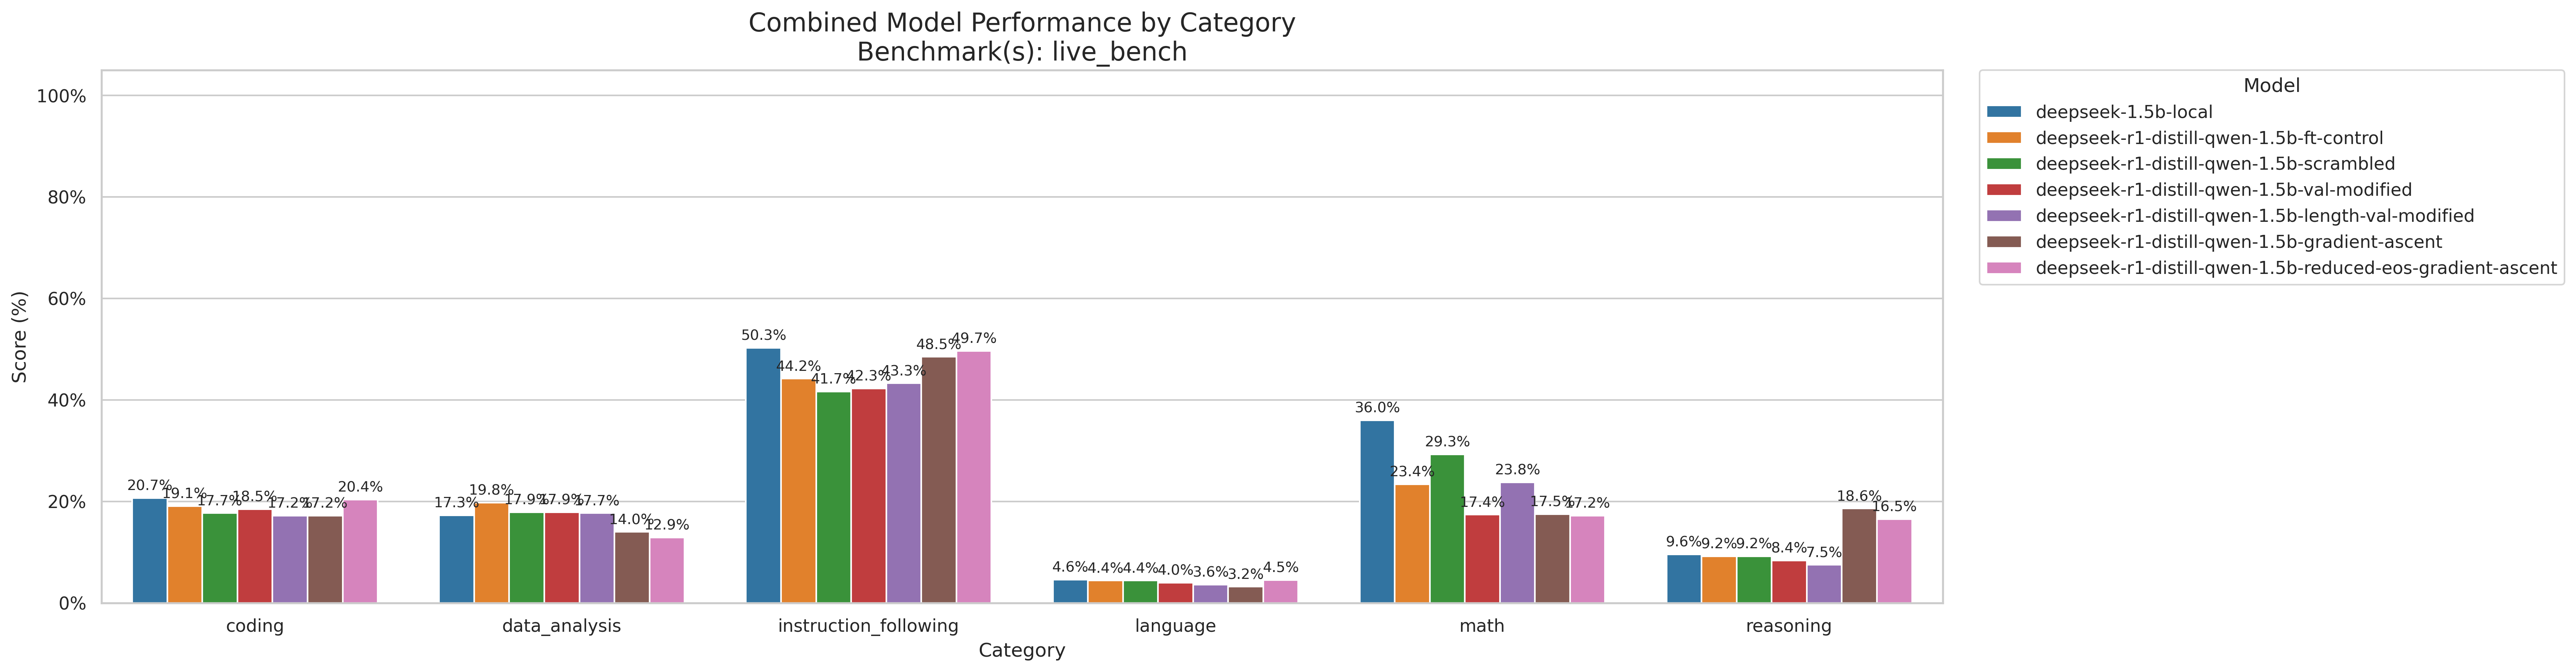
\includegraphics[width=0.9\linewidth]{combined_group_scores_live_bench.png}
    \caption{LiveBench benchmark results.}
    \label{fig:bench_and_direct}
\end{figure}
\begin{table}[h]
\centering
\tiny
\caption{Loss Values for Corrupted Dataset (Corr) and Gradient Ascent (Grad) by Topic}
\label{tab:loss}
\setlength{\tabcolsep}{3.5pt}
\begin{tabular}{|l|c|c|c|c|c|c|}
\hline
\textbf{Method} & \textbf{Coding} & \textbf{Data anal.} & \textbf{Instruct.} & \textbf{Lang.} & \textbf{Math} & \textbf{Reasoning} \\ \hline
Avg Accuracy (Corr) & 18.125 & 18.325 & 42.875 & 4.1 & 23.475 & 8.575 \\ \hline
Avg Accuracy (Grad) & 18.8 & 13.45 & 49.1 & 3.85 & 17.35 & 17.55 \\ \hline
Loss (Corr) & 2.575 & -1.025 & 7.425 & 0.5 & 12.525 & 1.025  \\ \hline
Loss (Grad) & 1.9 & 3.85 & 1.2 & 0.75 & 18.65 & -7.95  \\ \hline
\end{tabular}
\end{table}

As depicted in Figure 3 and shown in Table 1, there is a large decrease in math accuracy about 12.525\% from the corrupted dataset based unlearning, and about a 18.65\% decrease in math accuracy from the gradient ascent based unlearning. However, the total accuracy loss from performing gradient ascent is 18.4\%, while the accuracy loss from fine-tuning on the corrupted data set is 23.025\%. This means that performing gradient ascent made the model forget more about mathematics, while not having as much impact on other skills. Additionally, made clear in Table 1 we see very small decreases in accuracy in the Coding, Language, and Reasoning skill areas. This suggests that these areas are not very connected the the area of math in an LLM.
\begin{figure}[h]
    \centering
    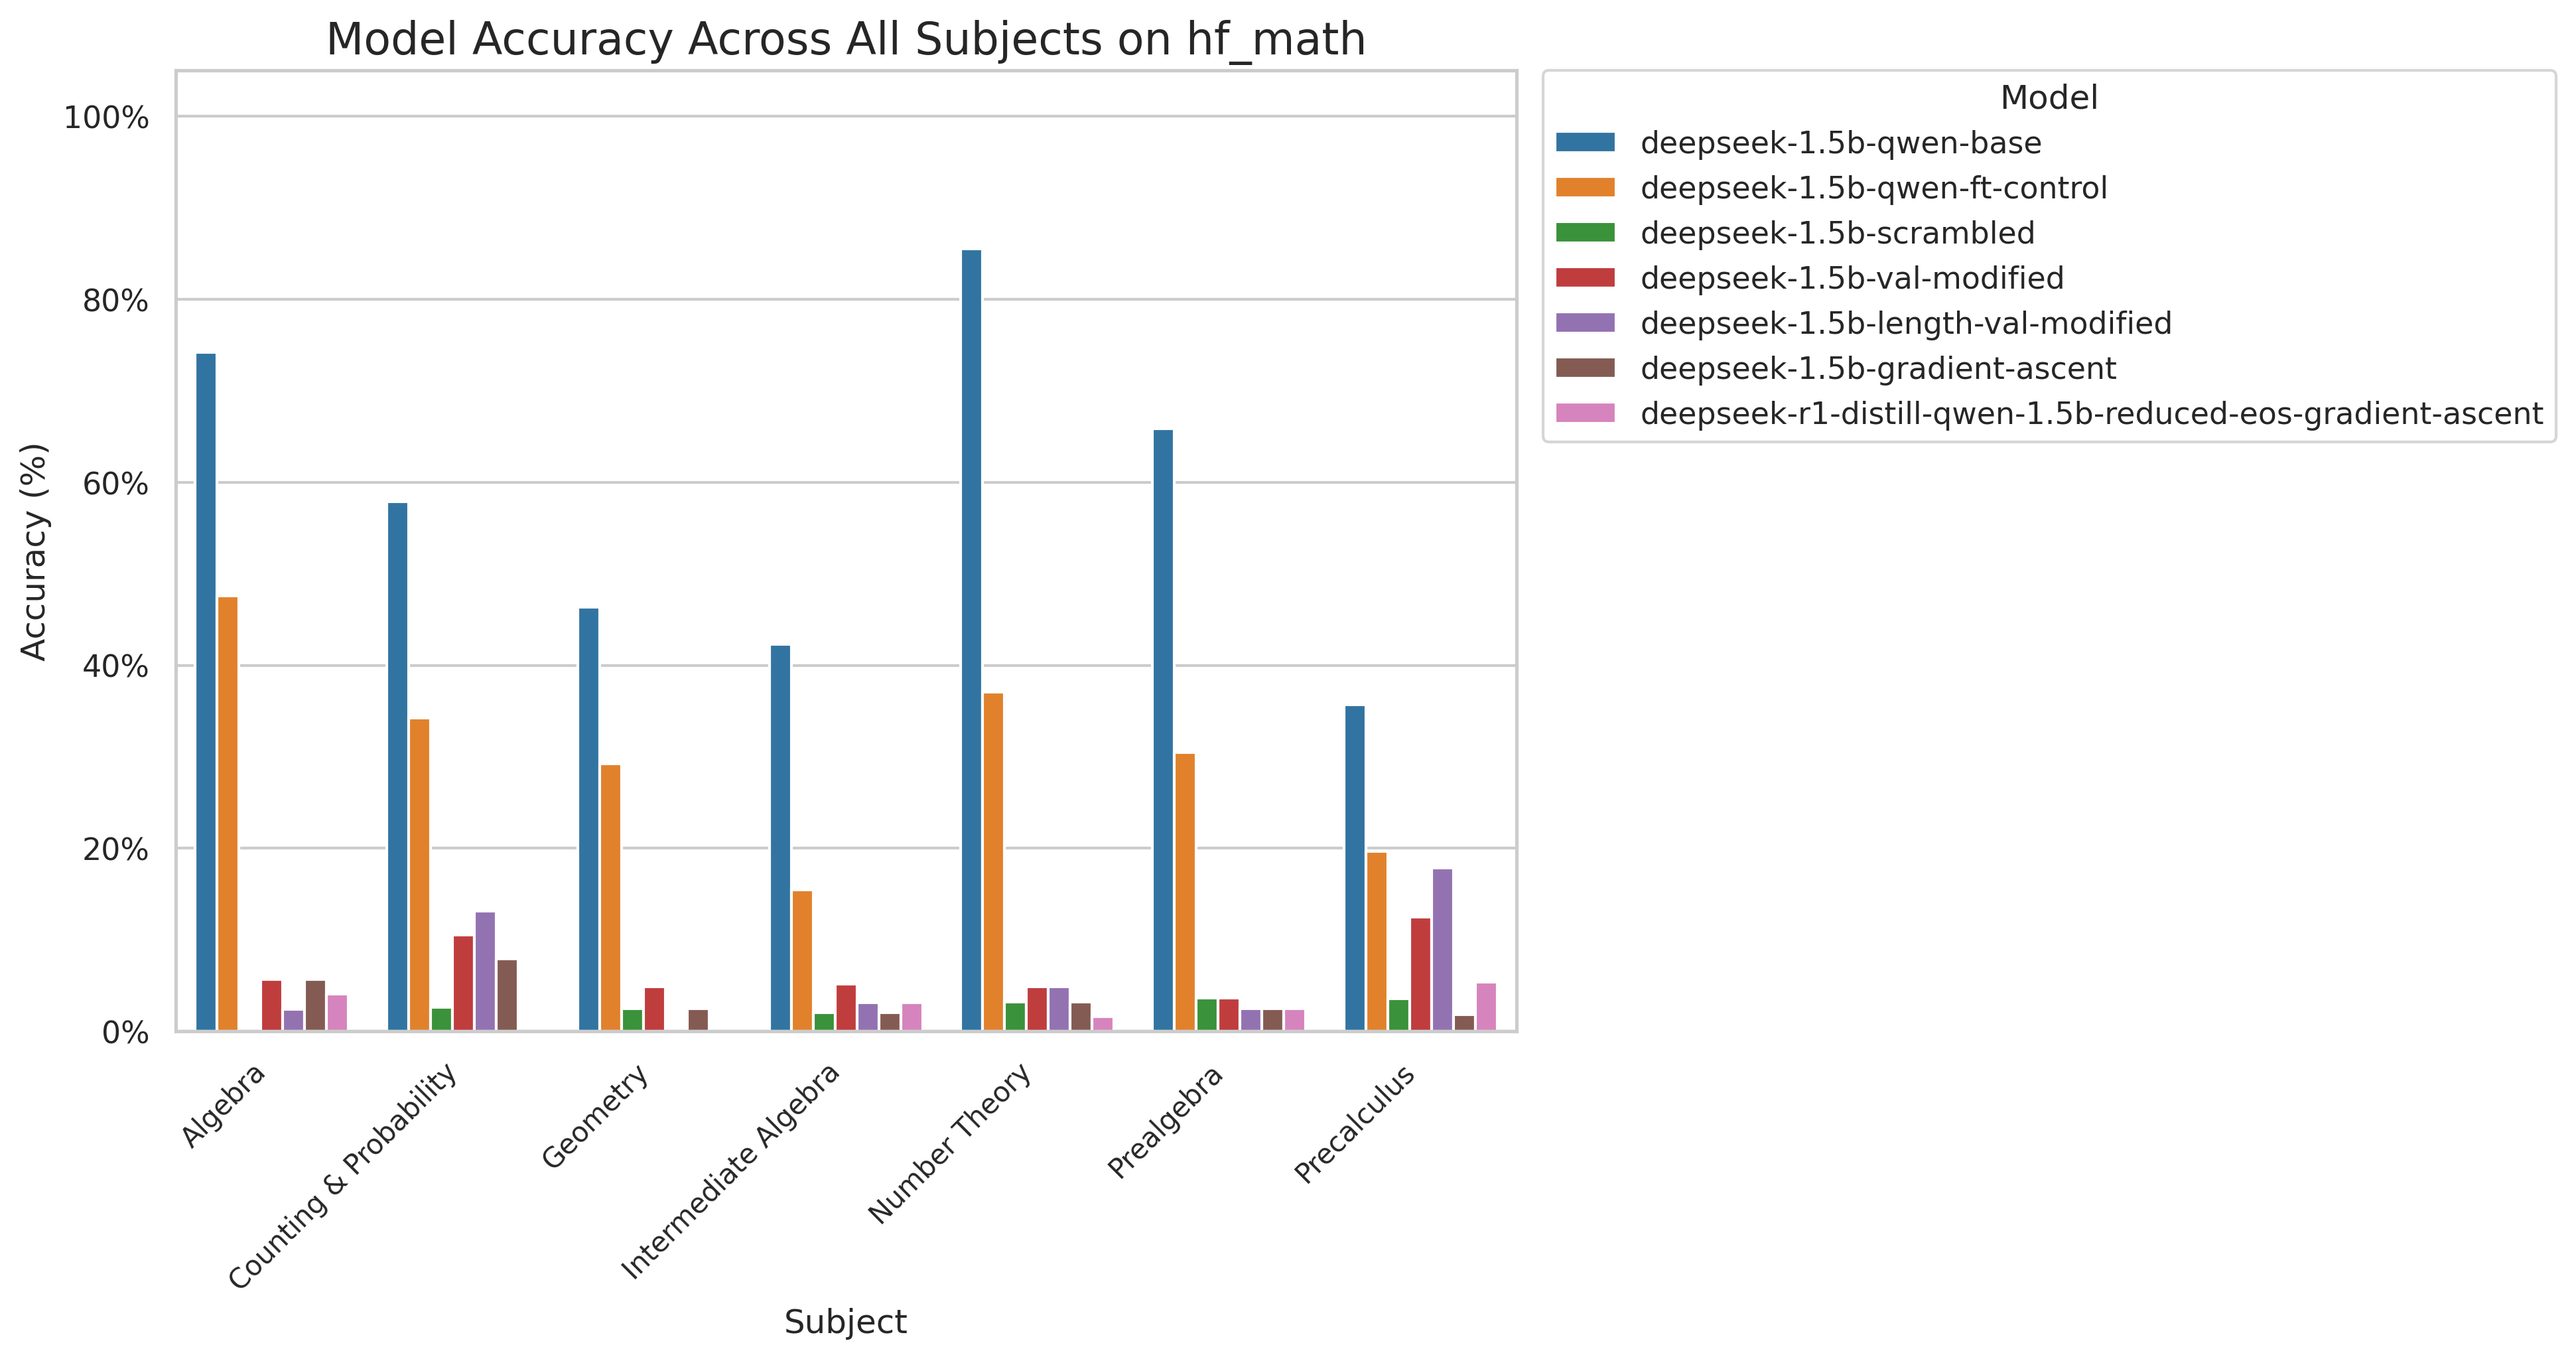
\includegraphics[width=0.9\linewidth]{main_prompt_hf_math_accuracy_all_subjects_combined_20250505_042444.png}
    \caption{Math500 accuracy with chain-of-thought prompting.}
    \label{fig:math500_cot}
\end{figure}
\begin{figure}[h]
    \centering
    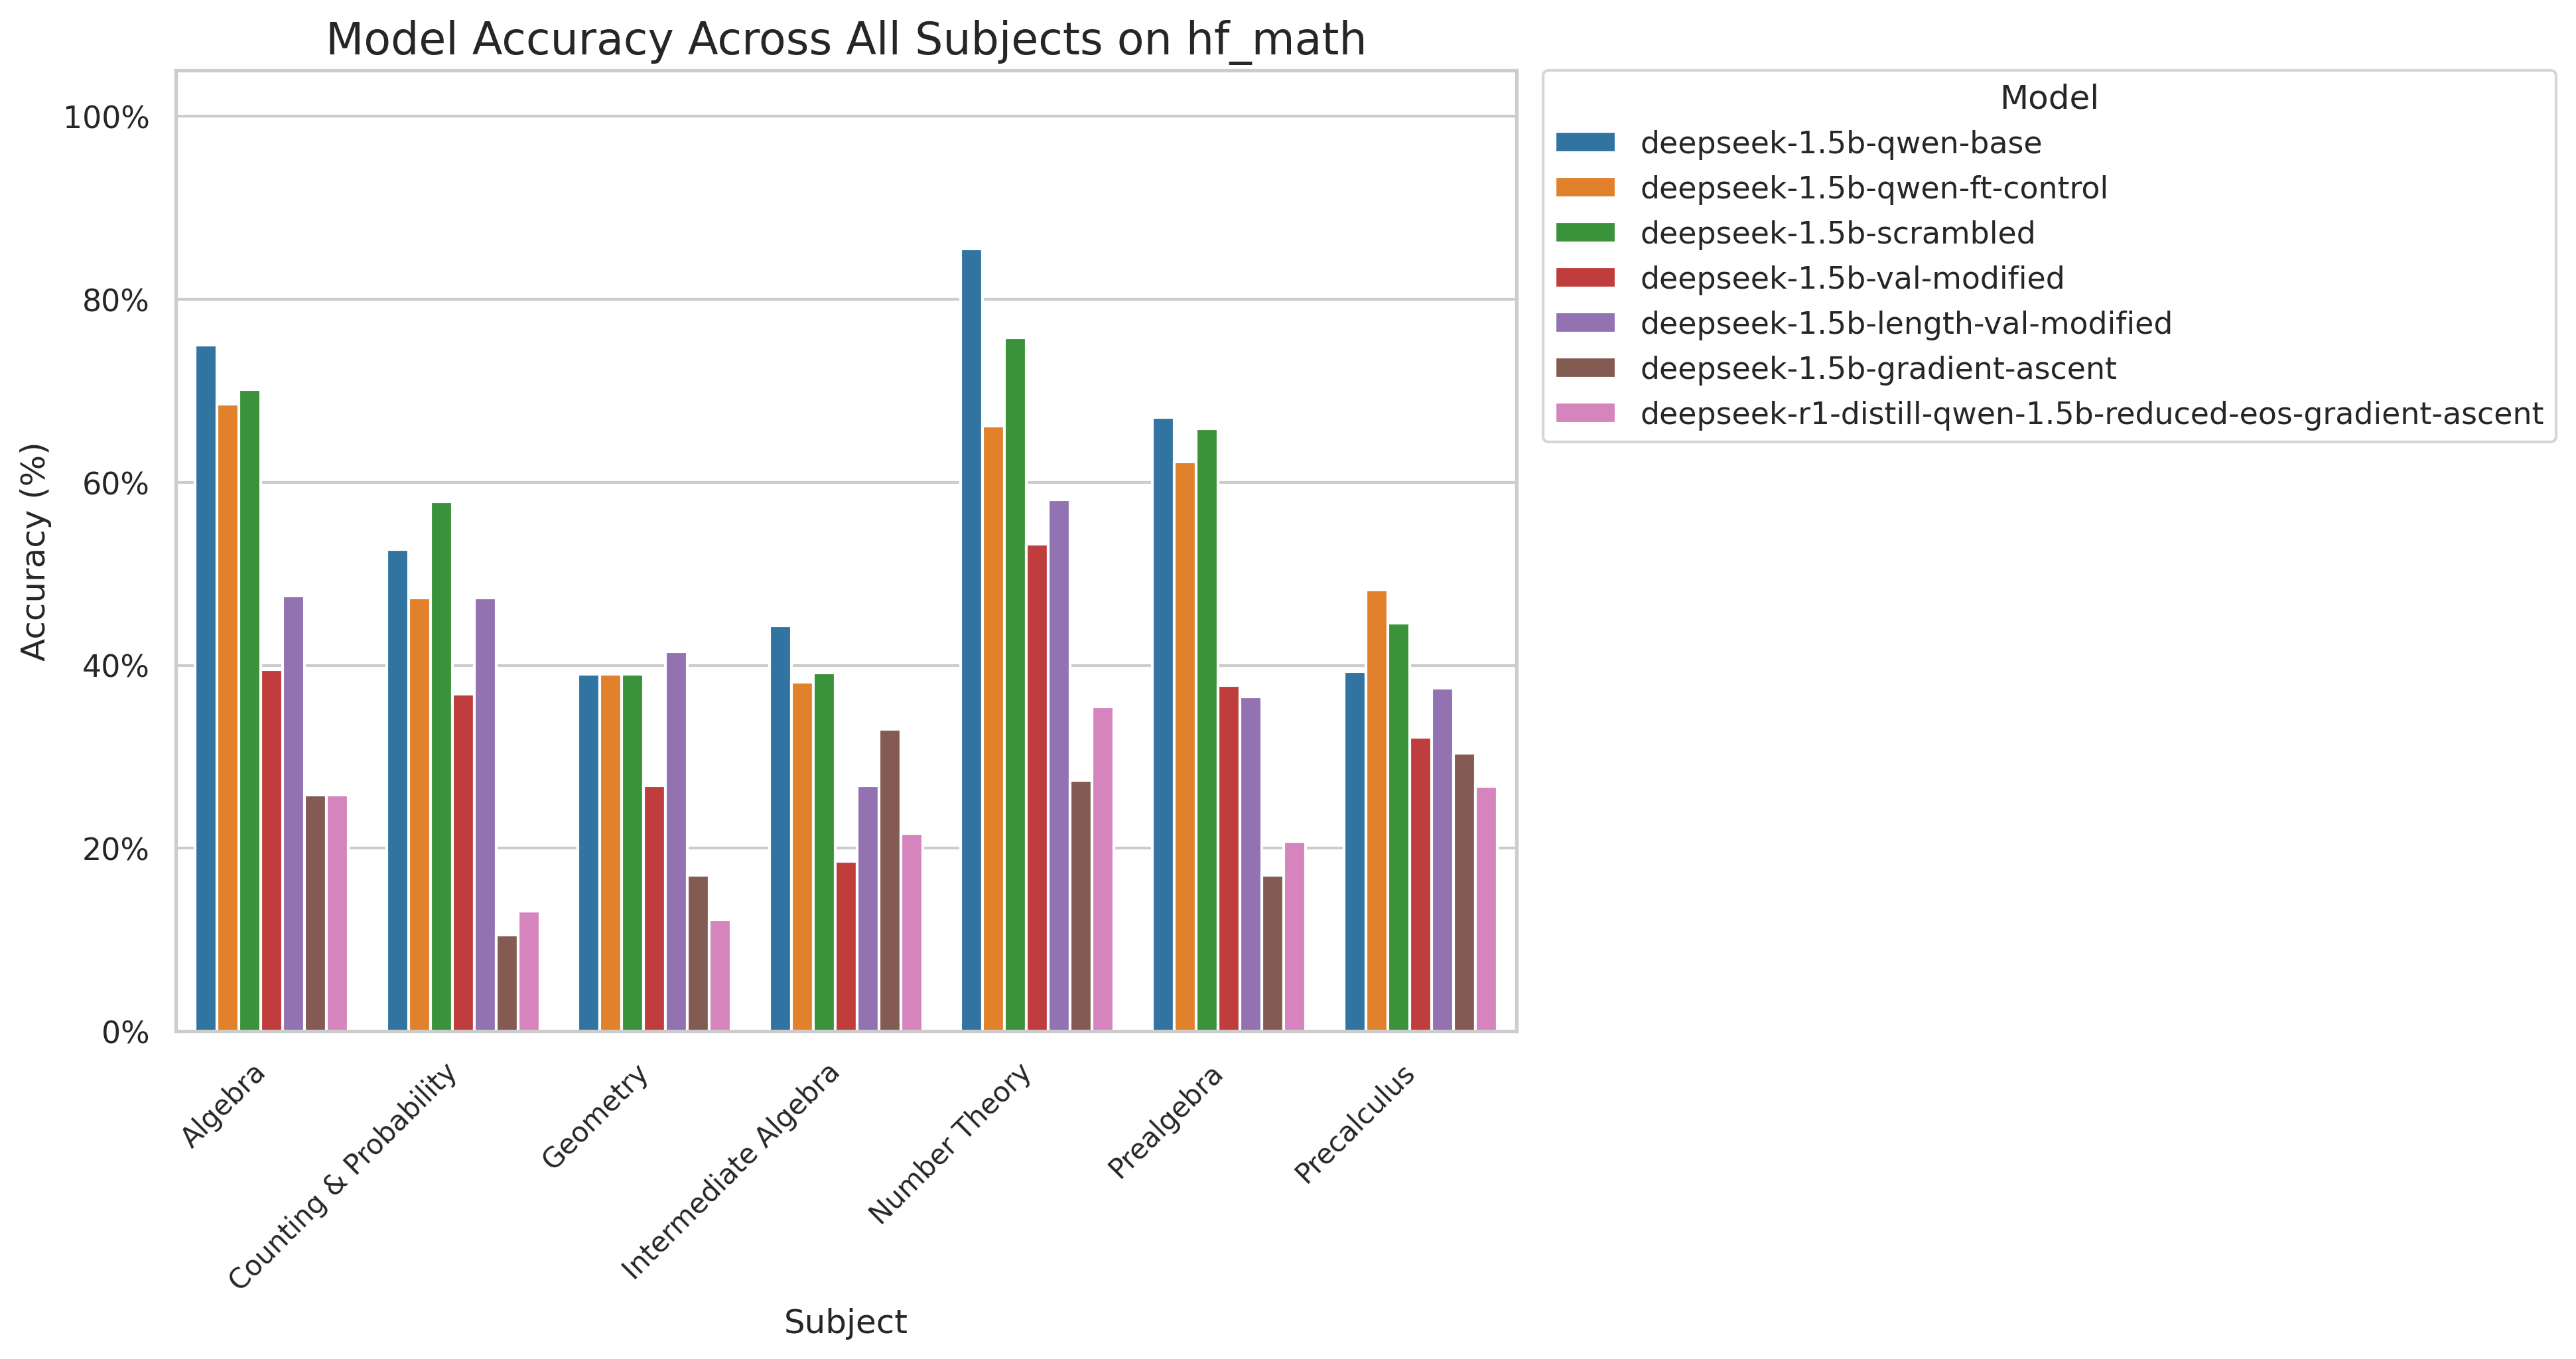
\includegraphics[width=0.9\linewidth]{new_prompt_hf_math_accuracy_all_subjects_combined_20250505_210815.png}
    \caption{Math500 accuracy without chain-of-thought prompting.}
    \label{fig:math500_cot}
\end{figure}

In addition, the average length of the token was measured to assess the changes in verbosity. It can be observed in Figure 6 that when gradient ascent is performed, the median token length for each response drops drastically, with a max of 87.426 decrease in median token length. This coupled with the model not losing much accuracy in the reasoning or instruction following category means that models with gradient ascent were able to give a correct answer while generating less tokens.
\begin{figure}[h]
    \centering
    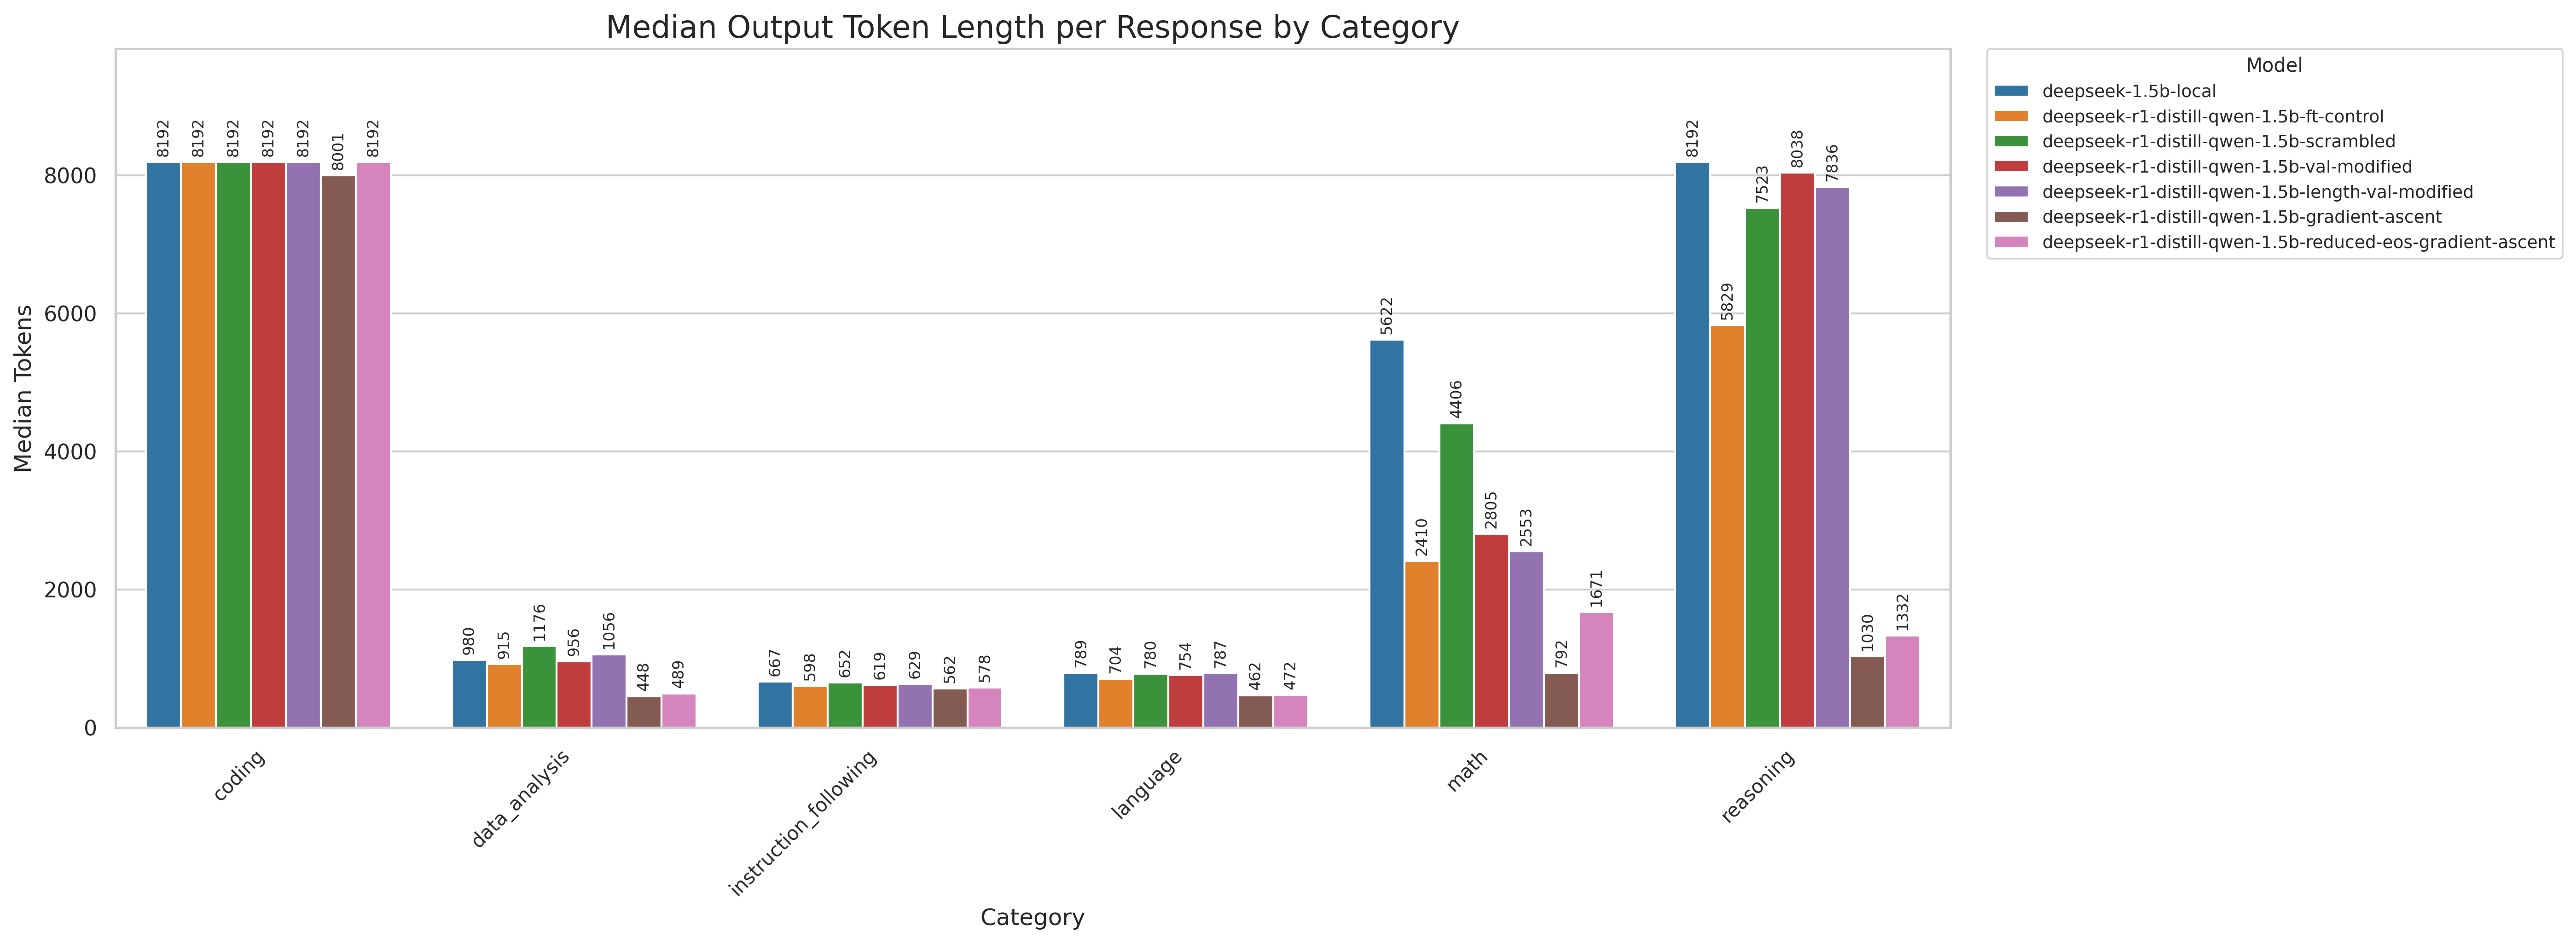
\includegraphics[width=1\linewidth]{token_length_median_by_category.png}
    \caption{Median token length per prompt category wise, from Livebench's benchmark}
    \label{fig:enter-label}
\end{figure}


\section{Discussion}
\subsection{Limitations}
In this study we only looked at deepseek-R1-qwen-1.5B, which is a relavitvley smaller model. Because of this, we do not know if these results will also appear in a very large LLM such as deepseek-R1. Additionally, we only use a subset of the questions in the prm dataset\cite{lightman2023lets}, therefore the converage for each math subject is limited.
\subsection{Future Considerations}
As described earlier, only one model was used deepseek-R1-qwen-1.5B. Future works should consider large models and different architectures. Additionally, only a few number of datasets and one LLM benchmark were used for testing. For higher converage, using more datasets or benchmarks should be considered.
\section{Conclusion}
In this report, the connectivity of different skill domains in LLMs was studied. This connectivity was studied by performing LLM unlearning on a specific skill domain, in this case mathematics. Unlearning was performed in two different forms: fine-tuning on a corrupted dataset and performing gradient ascent.


% Bibliography
\bibliographystyle{acl_natbib}
\bibliography{custom}

\end{document}
